\documentclass{mwhittaker}
\title{Deep RL Assignment 1}
\date{September 11, 2017}

\usepackage{graphicx}
\newcommand{\tabref}[1]{Table~\ref{tab:#1}}

\begin{document}
\maketitle

\begin{table}[h]
  \centering
  \begin{tabular}{|l|l|l|l|l|}
    \hline
                   & Mean Reward & Reward Stddev & Mean Reward & Reward Stddev \\
    Task           & (Expert)    & (Expert)      & (BC)        & (BC) \\\hline
    HalfCheetah-v1 & 4141.72     & 80.26         & 4012.04     & 199.79  \\\hline
    Reacher-v1     & -3.905      & 1.72          & -6.44       & 2.78 \\\hline
    Walker2d-v1    & 5517.27     & 72.15         & 1668.00     & 1624.38 \\\hline
  \end{tabular}
  \caption{
    Question 3.1. The mean and standard deviation reward of an expert policy
    and a policy learned via behavioral cloning (BC) on the HalfCheetah-v1,
    Reacher-v1, and Walker2d-v1 tasks. We see that the BC policy performs very
    well on HalfCheetah-v1, performs moderately well for Reacher-v1, and
    performs poorly on Walker2d-v1. Intuitively, errors in behavioral cloning
    do not seem to compound HalfCheetah-v1. In Reacher-v1, errors compound
    slightly. In Walker2d-v1, errors compound a lot; small mistakes can force
    the walker to fall over. Expert measurements for HalfCheetah-v1,
    Reacher-v1, and Walker2d-v1 were taken on 1500, 50000, and 1000 rollouts
    respectively. The BC models were trained on these rollouts and all
    measurements were taken on 100 rollouts. All three models were trained
    using a fully connected neural network with two hidden layers and the ReLU
    nonlinearity. The HalfCheetah-v1 model was trained with 32 neurons in both
    hidden layers for 105008 iterations of batch gradient descent. The
    Reacher-v1 model was trained with 64 neurons in both layers for 338953
    iterations. The Walker2d-v1 model was trained with 32 neurons in both
    layers for 93111 iterations. The Walker2d-v1 was trained for fewer
    iterations because its loss reached a fixpoint.
  }
  \label{tab:bc}
\end{table}

\begin{figure}[h]
  \centering
  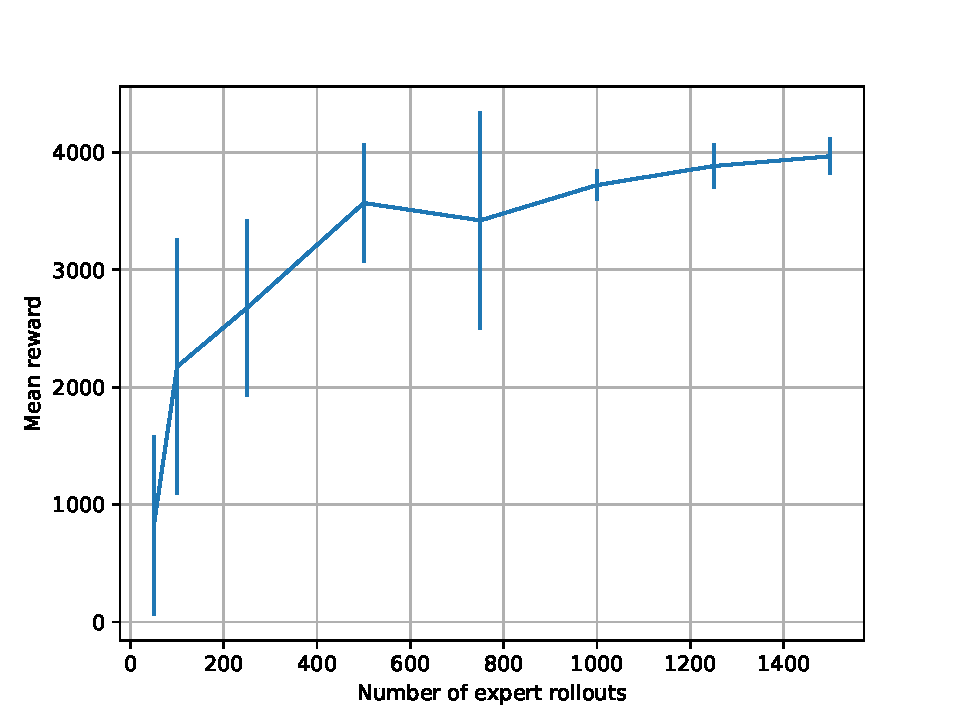
\includegraphics[width=\textwidth]{cheetah.pdf}
  \caption{
    The mean reward of a HalfCheetah-v1 BC model trained on various numbers of
    expert rollouts. Every BC model was trained using a fully connected
    two-layer neural network with the ReLU nonlinearity. There were 32 units in
    both hidden layers. Every model performed batch gradient descent with
    batches of 1000 for 5 full iterations through all provided expert rollouts.
    The graph also shows the standard deviation of the average return, measured
    on 100 rollouts. I decided to adjust the number of expert rollouts as a
    hyperparameter because for many applications, generating expert data can be
    the most expensive task, so it is interesting to see how much or how little
    expert data we actually need. For this assignment, expert data took up the
    most space (more than training checkpoints) so it was also nice to try and
    minimize the amount of rollouts stored.
  }
\end{figure}

\begin{figure}[h]
  \centering
  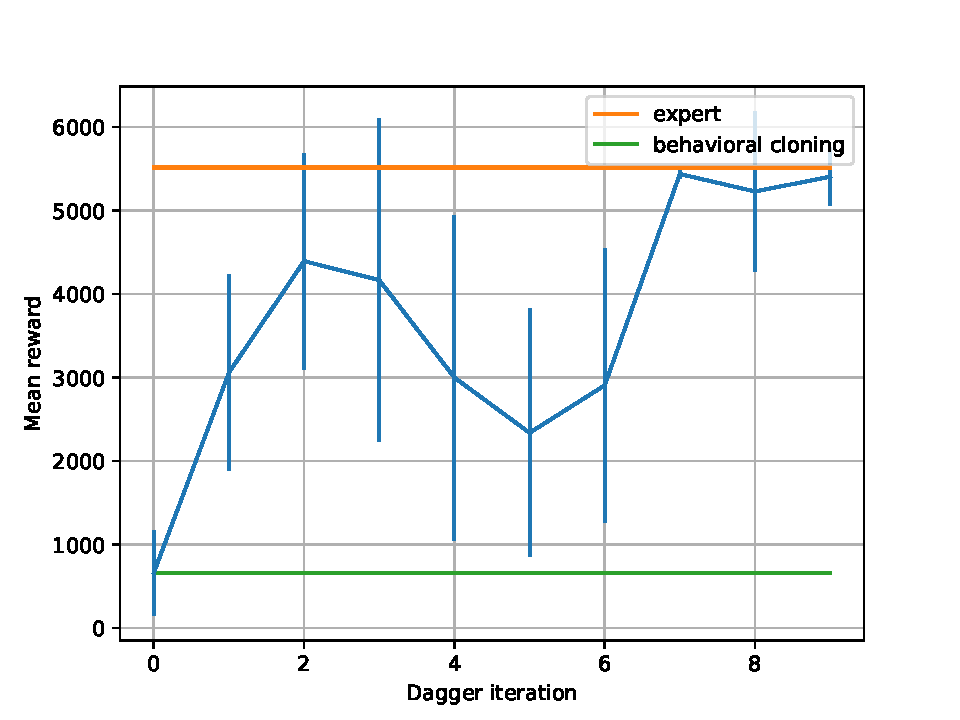
\includegraphics[width=\textwidth]{walker.pdf}
  \caption{
    Dagger performance for Walker2d-v1 task. The dagger model was built using
    the same neural network described in \tabref{bc} and was initialized with
    the same weights and the same 1000 expert rollouts. We perform 10
    iterations of dagger. Each iteration, we produce 100 new rollouts. We then
    train the model for 5000 iterations of batched gradient descent with
    batches of 10000. In green, we show the mean return of the iteration 0
    behavioral cloned model. In orange, we show the mean return of the expert
    as reported in \tabref{bc}. We see that dagger greatly improves the
    performance of the model making it almost as good as the expert after 10
    iterations.
  }
\end{figure}
\end{document}
